\chapter{Introduction}\label{cha:intro}


\begin{figure}[!htb]
 \begin{center}
%% psfrag: comment the following line if not using the psfrag package
  % \psfrag{pie makes me happy!}{$\pi$ makes me happy!}
%% includegraphics: comment the following if not using the graphicx package
  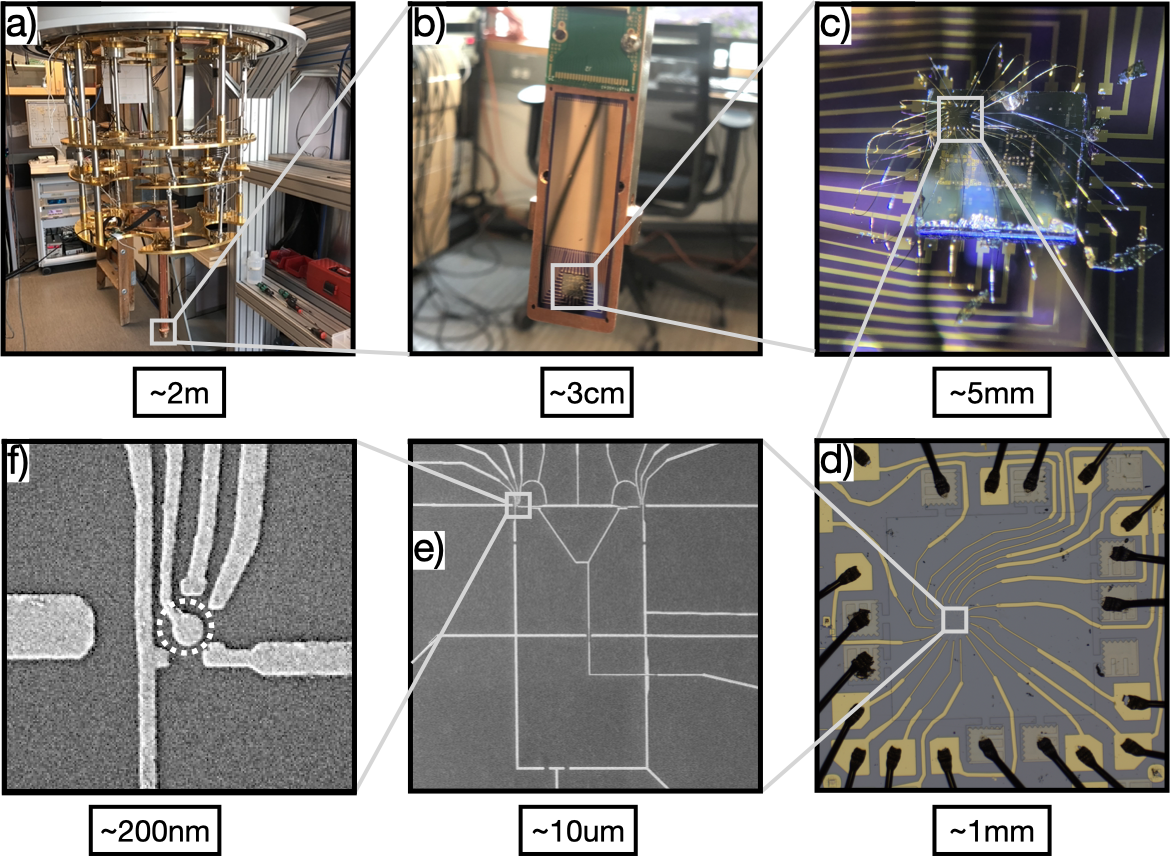
\includegraphics[width=1.0\textwidth]{figures/ch1/crop_FiguresMaster.001.png}
  \caption[Dilution fridge to quantum dot scale breakdown]{\label{fig:ch1/scale_breakdown} 
  % For some options that work with pdf\LaTeX, please see this discussion:
  %  \url{http://tex.stackexchange.com/questions/11839}. 
  Showing the various scales to connect how macro changes affect the nano. (\textbf{a}) A photograph of the Au plated cold plates in our dilution refrigerator. The lowest plate is called the mixing chamber and can reach \qty{7}{mK}. (\textbf{b}) A photograph of the Si chip carrier, onto which the heterostructure is stuck to. (\textbf{c}) An optical microscope image of the heterostructure stuck to the chip carrier. The thin wires are Al wire bonds which connect the device fabricated on the heterostructure to the fridge wires. (\textbf{d}) An optical microscope image of a single mesa on the heterostructure. A mesa is an isolated area of the heterostructure where we fabricate new designs. The black lines around the outside are the wire bonds and the bright Au are the thick (\qty{100}{nm}) `outer gates' which connect to the thin (\qty{10}{nm}) `inner gates'. (\textbf{d}) A scanning electron micrograph (SEM) of the inner gates. The mean free path of the electrons is of order \qty{3}{\mu m}. (\textbf{d}) An SEM image zoom in on the quantum dot. By carefully tuning the voltages on the inner gates, we can create an isolated puddle of electrons, typically with total occupation 0 - 10. 
   }
 \end{center}
\end{figure}


The Kondo effect first discovered in impure bulk metals in the 1930’s~\cite{de_haas} and explained later in the 1960’s~\cite{jun_kondo} has seen significant interest in the field of quantum devices. The high degree of tunability and control in these devices allows for testing predictions of the Anderson model~\cite{costi_kondo_mv_eo_regime}. In quantum devices, a Kondo state is engineered by strongly coupling a quantum dot with an overall spin (odd number of electrons) to two reservoirs. 

% Previous studies measure the conductance through the quantum dot and observe a zero bias peak in the middle of the Coulomb blockade valley. This effect requires strong coupling between the quantum dot and reservoirs.

% In this work, we reduce the coupling so the Kondo effect only enhances the conductance on the shoulder of the conductance peak. By simultaneously measuring the occupation of the quantum dot we can reliably show the small enhancement of conductance due to the Kondo effect. Measuring conductance and occupation at a range of temperatures allows for the determination of relevant parameters for comparison to Numerical Renormalisation Group (NRG) theory calculations. Good agreement is found at a range of coupling strengths. However, a discrepancy is found when the tunnel barriers to the quantum dot are tuned to be asymmetric. The strong asymmetric coupling approaches a regime where the quantum dot is coupled to a single lead. A regime where a recent measurement of the entropy of the Kondo effect found a discrepancy between data and NRG. Interestingly in our experiment, conductance data showed greater Kondo enhancement than NRG, whilst the previously measured entropy showed less Kondo enhancement than NRG. A direct comparison of conductance and entropy measured in the same device with similar settings is required to provide further enlightenment on this discrepancy. 

